\clearpage
\section{Sacred Vessels and Altar Linens}
\PCDPlateHeader{Plate III --- Sacred Vessels and Vessels for Communion}{Not to common scale}
\ifdefined\TriptychPrintEdition
\begin{center}
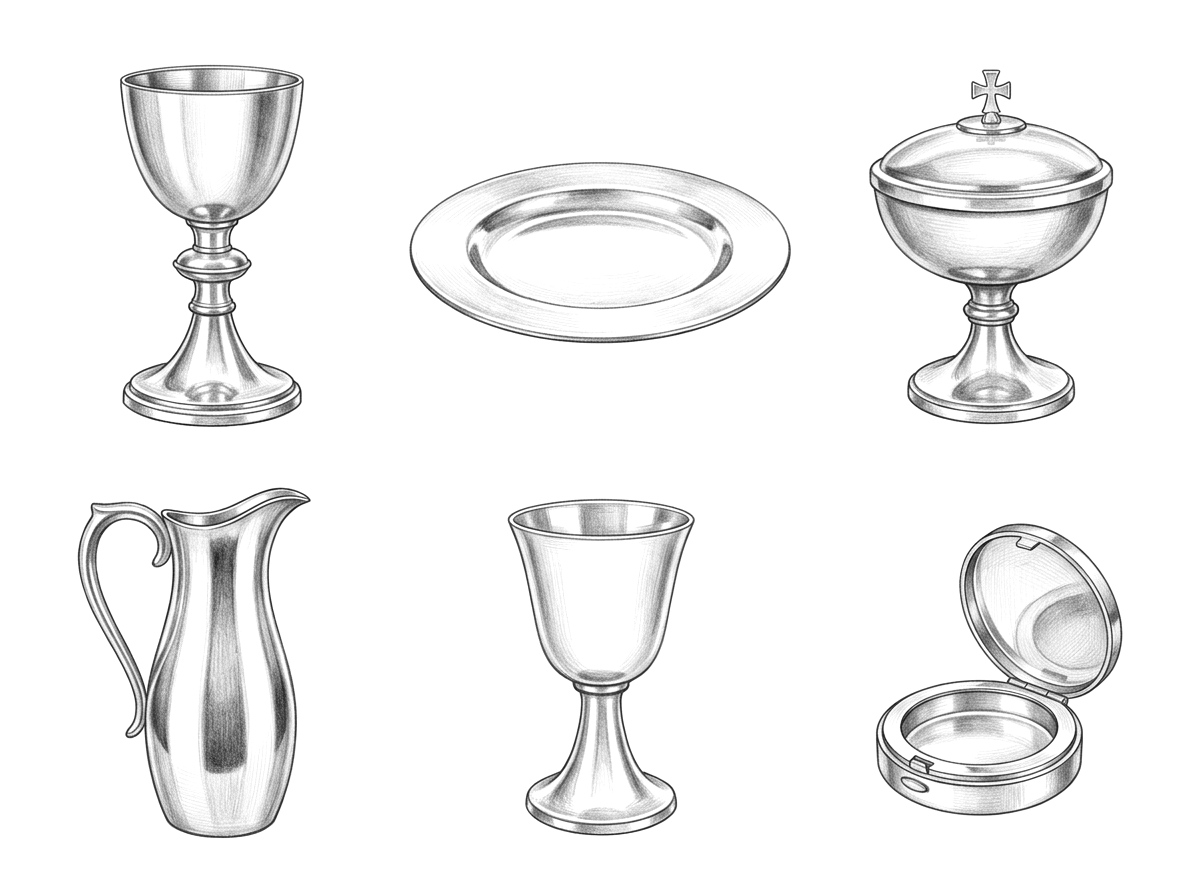
\includegraphics[width=0.92\linewidth,height=3.55in,keepaspectratio]{liturgy/roman-rite/postconciliar/2008-latin-2011-us-english/reference/roman-sanctuary-dictionary/shared/artwork/graphite/pc-art-03-sacred-vessels.png}
\end{center}
\PCDPositionKey{Top row, left to right: Chalice, wide shallow Paten, lidded footed Ciborium with cross finial. Bottom row, left to right: pitcher-style wine Flagon (pre-consecration transport only), footed Communion Cup (chalice), hinged pocket Pyx shown open.}
\else
\textbf{Visual Plate Summary (Plate III --- Sacred Vessels and Vessels for Communion, Not to common scale):} Six-vessel monochrome graphite comparison rendered with metallic reflections on white ground: top row left to right, a classical footed chalice with node, a broad shallow paten dish, and a lidded footed ciborium topped by a small cross; bottom row left to right, a tall slender pitcher-style wine flagon for bringing unconsecrated wine, a simpler footed Communion cup for distributing the Precious Blood, and a small hinged circular pocket pyx open to show its smooth gilded cavity.

\textbf{Reading order and object placement:} Top row, left to right: Chalice, wide shallow Paten, lidded footed Ciborium with cross finial. Bottom row, left to right: pitcher-style wine Flagon (pre-consecration transport only), footed Communion Cup (chalice), hinged pocket Pyx shown open.
\fi

\label{pc-obj-chalice}
\PCDEntryHead{Chalice}{Calix}{required}{N08}
\PCDField{Also called}{Principal Chalice; Eucharistic Chalice; \textit{Calix principalis}}
You may handle the chalice only while it is empty and unconsecrated---setting it neatly on the credence table before Mass and carrying it with both hands (one on the node, one steadying the top) to the altar at the Preparation of the Gifts when no deacon or instituted acolyte is serving. Once the Eucharistic Prayer begins, the chalice holds the Precious Blood of Christ: never touch it, never pour from it, never drink remaining drops, and never wash or wipe it afterward. Bring the water cruet for the priest, deacon, or instituted acolyte when they purify the chalice.

\PCDField{Where to look on the plate}{Top left (Plate III); center of the unfolded corporal (Plate X)}
\PCDField{Handling boundary}{\textbf{Server prepares or sets in place before or during Mass.} Servers may place the empty, unconsecrated chalice on the credence table before Mass and carry it to the altar at the Preparation of the Gifts if no deacon or instituted acolyte serves (GIRM 139). After consecration, servers never touch a chalice holding the Precious Blood, never consume from it, and never purify it (GIRM 279; RS 119; USCCB Norms 53). (Ordinary ministers: Bishop, Priest, Deacon.)}
\PCDSafety{Once consecrated, the chalice contains the Blood of Christ: servers and extraordinary ministers never purify it (strictly reserved to priest, deacon, or instituted acolyte), and remaining Precious Blood is never poured into the sacrarium or onto the ground (USCCB Norms 53--55).}
\PCDField{Do not confuse with}{Communion Cup, Ciborium, Flagon}
\PCDEntryRule

\label{pc-obj-paten}
\PCDEntryHead{Paten}{Patena}{required}{N09}
\PCDField{Also called}{Eucharistic Paten; Large Paten; \textit{Patena maior}}
Before the Eucharistic Prayer, you may carry the unconsecrated paten from the credence table to the altar if no deacon or instituted acolyte serves. Once the bread is consecrated, never touch the paten or attempt to brush particles off it. Do not confuse the Eucharistic paten with the Communion-plate (the handled plate held by a server under the chin of communicants): keep the Communion-plate steady and flat throughout distribution, and return it to the priest, deacon, or instituted acolyte for purification.

\PCDField{Where to look on the plate}{Top center (Plate III); front center of the unfolded corporal (Plate X)}
\PCDField{Handling boundary}{\textbf{Server prepares or sets in place before or during Mass.} Servers may bring the unconsecrated paten and hosts to the altar at the Preparation of the Gifts (GIRM 139) and hold the separate Communion-plate level under communicants' chins during distribution (GIRM 118c; RS 93). Servers never touch consecrated hosts on the paten and never purify either the paten or the Communion-plate after Communion (GIRM 278--279; RS 119). (Ordinary ministers: Bishop, Priest, Deacon.)}
\PCDSafety{If holding a Communion-plate during Holy Communion, keep it completely level beneath each communicant's chin without tipping it, and hand it back to the priest, deacon, or instituted acolyte at the altar or credence table so any particles are purified properly.}
\PCDField{Do not confuse with}{Ciborium, Pyx}
\PCDEntryRule

\label{pc-obj-ciborium}
\PCDEntryHead{Ciborium}{Pyxis}{provided}{N10}
\PCDField{Also called}{Host Vessel; Covered Ciborium; \textit{Ciborium}; \textit{Vas}}
Tell a ciborium from a chalice immediately by its wider, shallower bowl and its fitted domed lid topped with a small cross. You may carry an empty or unconsecrated ciborium to the altar at the Preparation of the Gifts or bring extra empty bowls at the Lamb of God when instructed. Once hosts are consecrated, or whenever a ciborium comes from the tabernacle, never open it, carry it, or wash it---only the priest, deacon, or instituted acolyte purifies sacred vessels, and extraordinary ministers approach the altar only after the priest communicates.

\PCDField{Where to look on the plate}{Top right (Plate III); draped in a white veil at rear right of the corporal (Plate X)}
\PCDField{Handling boundary}{\textbf{Server prepares or sets in place before or during Mass.} Servers may set empty, unconsecrated ciboria on the credence table before Mass and bring empty ciboria to the altar at the Preparation of the Gifts or Fraction Rite when directed (USCCB Norms 37). Servers never open the tabernacle, never carry a ciborium containing consecrated hosts, and never purify a ciborium after Communion (GIRM 279; RS 119). (Ordinary ministers: Bishop, Priest, Deacon, Instituted acolyte, Extraordinary minister of Holy Communion.)}
\PCDSafety{Never open, lift, or carry a ciborium containing the Blessed Sacrament unless ordained, instituted as an acolyte, or formally deputed as an extraordinary minister of Holy Communion for distribution; never wash an unpurified ciborium.}
\PCDField{Do not confuse with}{Chalice, Paten, Pyx}
\PCDEntryRule

\label{pc-obj-pyx}
\PCDEntryHead{Pyx}{Pyxis parva}{provided}{N11}
\PCDField{Also called}{Sick-Call Pyx; Pocket Pyx; \textit{Theca}; \textit{Pyxis}}
Look at the small round locket-box at the bottom right of Plate III: that is a pyx for bringing Holy Communion to the sick. You may pass an empty pyx to the priest before Mass if asked, but once a consecrated Host is placed inside it, only the priest, deacon, instituted acolyte, or a formally deputed extraordinary minister of Holy Communion may carry or open it. If you ever see a closed pyx left on the credence table or in the sacristy, do not open it---alert the priest immediately.

\PCDField{Where to look on the plate}{Bottom right, shown hinged open to display the recessed interior (Plate III)}
\PCDField{Handling boundary}{\textbf{Server recognizes only; does not handle.} Servers may hand an empty, clean pyx to a priest or deacon in the sacristy when requested, but never handle, carry, open, or purify a pyx containing a consecrated Host. (Ordinary ministers: Bishop, Priest, Deacon, Instituted acolyte, Extraordinary minister of Holy Communion.)}
\PCDSafety{A closed pyx may contain the Body of Christ. Never open an unattended pyx or place it in ordinary storage; report any closed pyx found in the sanctuary or sacristy immediately to the priest or deacon.}
\PCDField{Do not confuse with}{Ciborium, Paten}
\PCDEntryRule

\label{pc-obj-communion-cup}
\PCDEntryHead{Communion Cup}{Calix}{territorial adaptation}{N12}
\PCDField{Also called}{Communion Chalice; Additional Chalice; \textit{Calix ad Communionem sub utraque specie}}
Communion cups are smaller, simpler chalices used when the congregation receives the Precious Blood. You may place empty Communion cups and clean purificators on the credence table before Mass and carry empty cups to the altar at the Preparation of the Gifts so the priest or deacon can fill them with wine before the Eucharistic Prayer. Once Mass enters the Eucharistic Prayer, never touch any Communion cup, never pour wine or Precious Blood into one, and never wash or wipe them after Communion.

\PCDField{Where to look on the plate}{Bottom center (Plate III); flanking the principal chalice beside folded purificators (Plate X)}
\PCDField{Handling boundary}{\textbf{Server prepares or sets in place before or during Mass.} Servers may set empty, clean Communion cups and folded purificators on the credence table before Mass and carry empty cups to the altar at the Preparation of the Gifts before consecration. Once the Eucharistic Prayer begins, servers never touch, carry, consume from, or purify Communion cups (GIRM 279; RS 119; USCCB Norms 53). (Ordinary ministers: Bishop, Priest, Deacon, Instituted acolyte, Extraordinary minister of Holy Communion.)}
\PCDSafety{Strict liturgical law: wine must be poured into Communion cups before consecration---never pour the consecrated Precious Blood from a flagon or between chalices (RS 106). Following the October 2006 non-renewal of the temporary U.S. indult, extraordinary ministers and altar servers never purify Communion cups; purification is reserved strictly to priest, deacon, or instituted acolyte (USCCB Norms 53).}
\PCDField{Do not confuse with}{Chalice, Flagon, Ciborium}
\PCDEntryRule

\label{pc-obj-cruets}
\PCDEntryHead{Cruets}{Urceoli}{required}{N13}
\PCDField{Also called}{Wine and Water Cruets; \textit{Ampullae}; \textit{Urceoli cum vino et aqua}}
Cruets are among the most frequent items you will handle at Mass. Check before Mass that you know which holds wine and which holds water---clear glass makes this easy. Leave the stoppers safely on the credence tray, carry the cruets steadily to the side of the altar at the Preparation of the Gifts with handles turned toward the priest or deacon (wine first, then water), bow when stepping back, and return them immediately to the credence table. After Communion, bring the water cruet promptly for the priest, deacon, or instituted acolyte to purify the sacred vessels.

\PCDField{Where to look on the plate}{See Plate VI, top left (paired with stoppers on an oval metal tray); Plate I, atop the credence table}
\PCDField{Handling boundary}{\textbf{Server carries and presents to priest or deacon.} Cruets are core altar-server equipment: servers prepare them cleanly on the credence table, carry them to the altar with stoppers removed and handles turned toward the priest or deacon, return them promptly off the altar mensa (GIRM 306), and bring the water cruet back for vessel purification after Communion. (Ordinary ministers: Priest, Deacon, Instituted acolyte, Altar server.)}
\PCDSafety{Remove glass stoppers safely on the credence table before approaching the altar so stoppers are not dropped on stone steps; never leave cruets sitting on the altar table during the Eucharistic Prayer (GIRM 306).}
\PCDField{Do not confuse with}{Flagon, Lavabo Towel}
\PCDEntryRule

\label{pc-obj-flagon}
\PCDEntryHead{Flagon}{Lagoena}{permitted}{N14}
\PCDField{Also called}{Wine Pitcher; Offertory Carafe; \textit{Lagena}; \textit{Ampulla maior}}
A flagon is simply a large wine pitcher used to bring unconsecrated wine up the aisle in the Procession of the Gifts when many Communion cups are needed. Receive it cleanly from the priest or deacon at the sanctuary steps, bring it to the altar so the priest or deacon can pour all the wine into the chalices before the Eucharistic Prayer starts, and immediately carry the empty flagon back to the credence table. A flagon must never remain on the altar during the consecration (RS 106).

\PCDField{Where to look on the plate}{Bottom left, tall slender pitcher with curved handle and pouring lip (Plate III)}
\PCDField{Handling boundary}{\textbf{Server handles directly.} Servers may set the flagon at the gifts table before Mass, receive the unconsecrated flagon from the priest or deacon at the foot of the altar, and remove the empty flagon promptly from the altar to the credence table before the Eucharistic Prayer begins. (Ordinary ministers: Faithful, Priest, Deacon, Instituted acolyte, Altar server.)}
\PCDSafety{Strict liturgical boundary (Redemptionis Sacramentum 106): never leave a flagon containing wine on the altar during the Eucharistic Prayer, never treat a flagon as a chalice, and never allow the consecrated Precious Blood to be poured from a flagon into Communion cups.}
\PCDField{Do not confuse with}{Chalice, Communion Cup, Cruets}
\PCDEntryRule

\clearpage
\subsection{Altar and Vessel Linens}
\PCDPlateHeader{Plate IV --- Altar and Vessel Linens}{Not to common scale}
\ifdefined\TriptychPrintEdition
\begin{center}
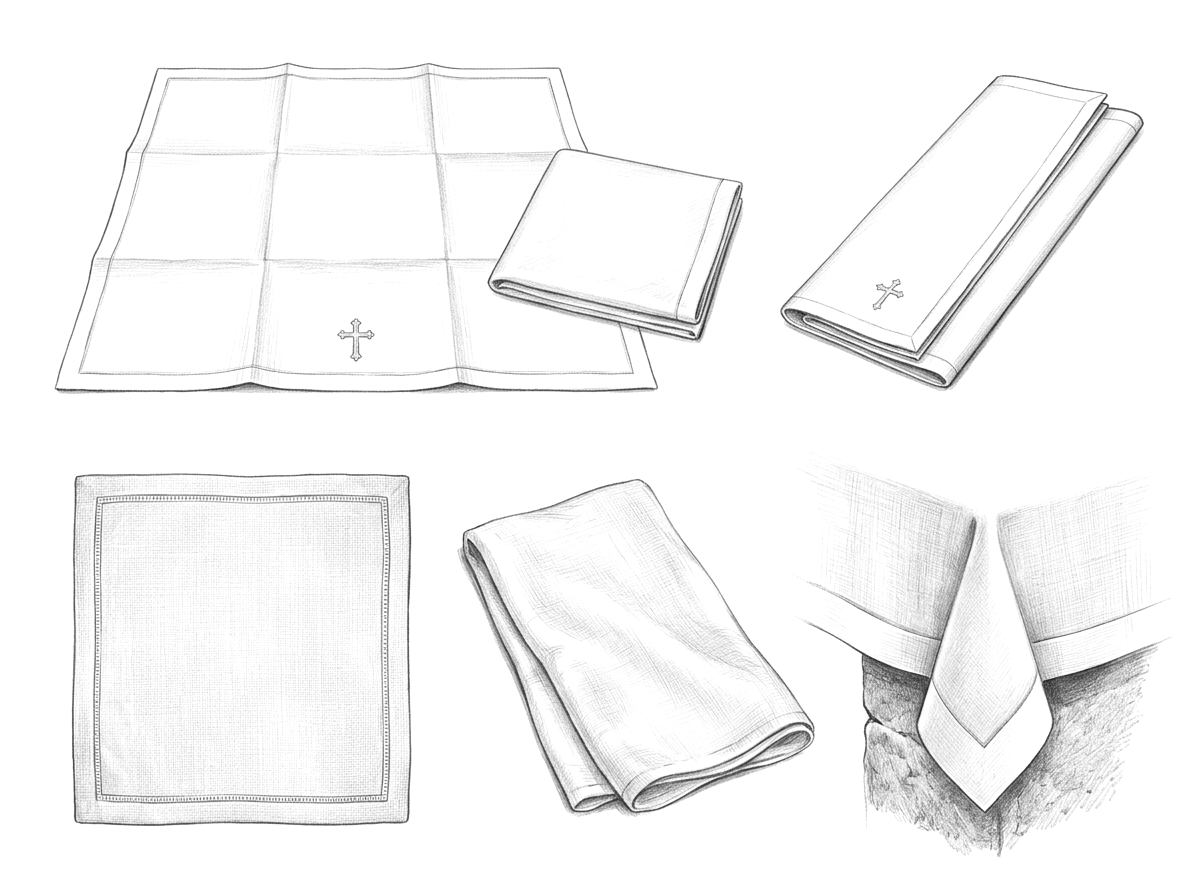
\includegraphics[width=0.92\linewidth,height=3.55in,keepaspectratio]{liturgy/roman-rite/postconciliar/2008-latin-2011-us-english/reference/roman-sanctuary-dictionary/shared/artwork/graphite/pc-art-04-white-linens.png}
\end{center}
\PCDPositionKey{Top left: unfolded square Corporal showing its three-by-three fold grid and front stitched cross, paired with a folded Corporal; top right: oblong Purificator folded lengthwise in thirds with stitched cross visible near the lower folded end; bottom left: stiffened square Pall; bottom center: folded Lavabo Towel; bottom right: hemmed corner of white Altar Cloth draped over the mensa.}
\else
\textbf{Visual Plate Summary (Plate IV --- Altar and Vessel Linens, Not to common scale):} Five-subject monochrome graphite textile study on pure white stock differentiating white altar linens by crease geometry and drape: top left, an unfolded square corporal creased into nine squares with a small stitched cross near the front center edge beside a folded square corporal; top right, an oblong purificator folded lengthwise in thirds with a small stitched cross visible near the lower folded end; bottom left, a rigid flat square linen pall; bottom center, a softly folded rectangular lavabo finger towel; bottom right, a hemmed corner of a white altar cloth hanging over a stone altar edge.

\textbf{Reading order and object placement:} Top left: unfolded square Corporal showing its three-by-three fold grid and front stitched cross, paired with a folded Corporal; top right: oblong Purificator folded lengthwise in thirds with stitched cross visible near the lower folded end; bottom left: stiffened square Pall; bottom center: folded Lavabo Towel; bottom right: hemmed corner of white Altar Cloth draped over the mensa.
\fi

\label{pc-obj-altar-cloth}
\PCDEntryHead{Altar Cloth}{Mappa}{required}{N15}
\PCDField{Also called}{Fair linen; Altar linen; \textit{Mappa altaris}; \textit{Mappae}; \textit{Tobalea}}
Look at bottom right of Plate IV and across the altar on Plates I and II: the smooth white altar cloth covers the mensa for every Mass. If asked to help smooth or lay a fresh cloth before Mass, make sure your hands are spotless and never lean on the covered altar. When extinguishing altar candles after Mass, use a snuffer so hot wax never splatters on the white linen. If a drop of the Precious Blood ever falls onto the altar cloth, never try to wipe it yourself---alert the priest or deacon right away.

\PCDField{Where to look on the plate}{Bottom right corner drape (Plate IV); dressing the altar (Plates I--II)}
\PCDField{Handling boundary}{\textbf{Server prepares or sets in place before or during Mass.} Servers may assist the sacristan in laying or smoothing a clean altar cloth before Mass with clean hands, keeping wax, ink, and unauthorized items off the mensa and reporting any spill of the Precious Blood immediately to the priest or deacon. (Ordinary ministers: Bishop, Priest, Deacon.)}
\PCDSafety{Never blot or wash a spill of the Precious Blood on the altar cloth yourself; notify the priest or deacon at once so the spot is washed with water and the ablution poured into the sacrarium (GIRM 280; RS 120). Guard the linen against candle flames and molten wax.}
\PCDField{Do not confuse with}{Corporal, Lavabo Towel}
\PCDEntryRule

\label{pc-obj-corporal}
\PCDEntryHead{Corporal}{Corporale}{required}{N16}
\PCDField{Also called}{Altar corporal; \textit{Palla corporalis}}
Recognize the corporal on Plate IV by its square shape, crisp nine-square fold grid, and small cross near the front edge---never confuse it with the narrow triple-folded purificator or the soft lavabo towel. Before Mass, set the clean folded corporal on the credence table; at the Preparation of the Gifts, carry it neatly to the altar if no deacon or instituted acolyte is serving. Once consecrated hosts have rested upon it, never snap, shake, or pick it up casually; let the priest, deacon, or instituted acolyte fold it inward, and carry it flat only if instructed.

\PCDField{Where to look on the plate}{Top left, shown unfolded in a 3x3 crease grid and folded beside it (Plate IV); beneath vessels (Plate X)}
\PCDField{Handling boundary}{\textbf{Server prepares or sets in place before or during Mass.} Servers may set a clean, folded corporal on the credence table before Mass and bring it to the altar at the Preparation of the Gifts when no deacon or instituted acolyte serves; after consecration, servers never shake, refold carelessly, or wash a used corporal, and move a folded corporal flat and level only when directed after purification. (Ordinary ministers: Bishop, Priest, Deacon, Instituted acolyte.)}
\PCDSafety{A used corporal may hold fine particles of the Sacred Host. Never shake it out or wash it directly in an ordinary sink; first soak and hand-rinse it in a dedicated basin and pour that first rinse water into the sacrarium or directly into clean earth before ordinary laundering (RS 120).}
\PCDField{Do not confuse with}{Purificator, Pall, Lavabo Towel, Altar Cloth}
\PCDEntryRule

\label{pc-obj-purificator}
\PCDEntryHead{Purificator}{Purificatorium}{required}{N17}
\PCDField{Also called}{Chalice cloth}
Spot the purificator at top right of Plate IV by its narrow triple-folded shape and small embroidered cross---never mix it up with the plain, uncrossed lavabo towel. Before Mass, lay clean purificators beside the unconsecrated chalices on the credence table and bring them to the altar at the Preparation of the Gifts if asked. Once Communion begins, used purificators carry traces of the Precious Blood; never wipe chalices with them, never shake them out, and leave them with the priest, deacon, or instituted acolyte for proper care after purification.

\PCDField{Where to look on the plate}{Top right, folded lengthwise in thirds with stitched cross visible near the lower folded end (Plate IV); beside Communion cups (Plate X)}
\PCDField{Handling boundary}{\textbf{Server prepares or sets in place before or during Mass.} Servers may set clean, unused purificators on the credence table before Mass and carry them with unconsecrated chalices at the Preparation of the Gifts; once used with the Precious Blood, servers never wipe sacred vessels with them, shake them, or place them in ordinary laundry. (Ordinary ministers: Bishop, Priest, Deacon, Instituted acolyte, Extraordinary minister of Holy Communion.)}
\PCDSafety{Used purificators hold traces of the Precious Blood. Never wash a used purificator in an ordinary sink or mix it into regular laundry; soak and hand-rinse it first in a dedicated basin and pour that first rinse water into the sacrarium or directly into clean earth before ordinary laundering (RS 120).}
\PCDField{Do not confuse with}{Lavabo Towel, Corporal, Pall}
\PCDEntryRule

\label{pc-obj-pall}
\PCDEntryHead{Pall}{Palla}{optional}{N18}
\PCDField{Also called}{Chalice pall; \textit{Palla calicis}}
Look at bottom left of Plate IV: unlike the folded corporal above it, the pall is completely flat and stiff so it rests steadily across the chalice rim without sagging into the wine. If your parish uses a pall, set it cleanly atop the paten on the unconsecrated chalice at the credence table and carry it steadily to the altar at the Preparation of the Gifts. Once the Eucharistic Prayer begins, leave placing and removing the pall to the priest or deacon.

\PCDField{Where to look on the plate}{Bottom left, stiffened square (Plate IV)}
\PCDField{Handling boundary}{\textbf{Server prepares or sets in place before or during Mass.} Servers may set a clean pall atop the unconsecrated chalice on the credence table and bring it to the altar at the Preparation of the Gifts; once the Eucharistic Prayer begins, servers do not place or remove the pall over a chalice containing the Precious Blood. (Ordinary ministers: Bishop, Priest, Deacon.)}
\PCDSafety{Remove any rigid insert before washing a slipcover pall; if drops of the Precious Blood ever touch the linen underside, soak and hand-rinse the linen first into the sacrarium or clean earth before ordinary laundering (RS 120).}
\PCDField{Do not confuse with}{Corporal, Purificator}
\PCDEntryRule

\label{pc-obj-lavabo-towel}
\PCDEntryHead{Lavabo Towel}{Manutergium}{required}{N19}
\PCDField{Also called}{Finger towel; Hand towel; \textit{Tersorium}}
Presenting the lavabo is one of your core server ministries at the Preparation of the Gifts. Spot the lavabo towel at bottom center of Plate IV by its soft, unstarched folds and lack of a stitched cross---never grab a purificator by mistake. Bring the water pitcher, shallow basin, and unfolded towel to the side of the altar (draping the towel cleanly over your forearm if serving alone, or holding it wide between both hands when two servers assist), bow to the priest, pour a steady gentle stream over his fingers into the basin, offer the towel cleanly, bow again, and return all items to the credence table.

\PCDField{Where to look on the plate}{Bottom center, softly folded rectangular cloth (Plate IV); paired with lavabo pitcher and basin (Plate VI)}
\PCDField{Handling boundary}{\textbf{Server carries and presents to priest or deacon.} Servers prepare the lavabo towel on the credence table before Mass, carry it with the water pitcher and basin to the side of the altar at the Preparation of the Gifts, present it cleanly unfolded for the priest to dry his hands, bow before and after, and return all three items promptly to the credence table. (Ordinary ministers: Bishop, Priest.)}
\PCDSafety{Keep plain lavabo towels strictly separate from sacred purificators in both the sacristy and credence setup so the two are never interchanged. Hold the pitcher and basin level so water does not splash onto the altar cloth or sanctuary steps.}
\PCDField{Do not confuse with}{Purificator, Corporal}
\PCDEntryRule
